\section{Design}
In this section, we describe the three modules of \TheName{}, i.e. 
Monitor, Locator, and Mitigator. Figure~\ref{fig:architecture} shows the architecture of our design. 
Monitor collects the aggregated throughputs of TCP flows for each port of switches by installing flow rules. 
%Monitor collects the aggregated throughputs of TCP flows existing each port of switches by installing flow rules
Once the aggregated throughput of a switch degrades significantly, Locator will be triggered by Monitor which suspect a low-rate TCP attack. Then Locator will begin to confirm and locate the attack sources according to the statistics of the abnormal port. Finally, Locator informs Mitigator of the attack source information, and Mitigator will install flow rules on the related switch to eliminate the influence of the low-rate TCP attack. 


\begin{figure}
\vspace{0in}
\centering
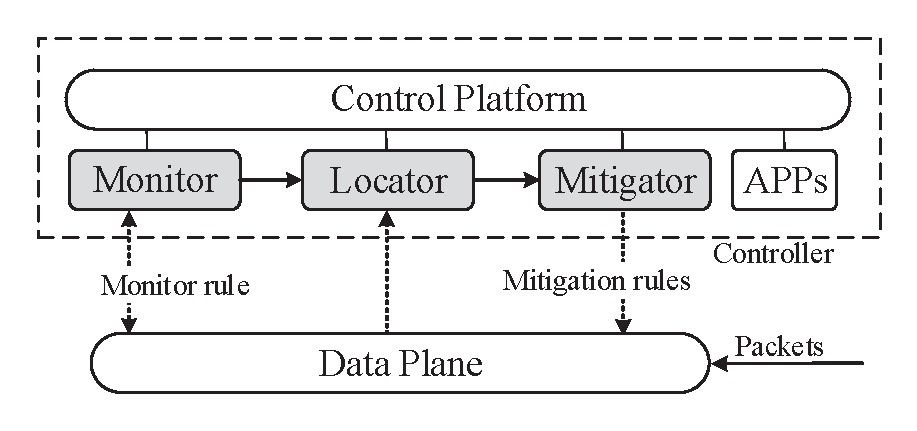
\includegraphics[width=3.4in]{Design/architecture.pdf}
\vspace{-0.1in}
\caption{\small{The architecture of our design.}}
\label{fig:architecture}
\vspace{-0.2in}
\end{figure}


\subsection{Monitor Module}
Monitor aims at detecting possible low-rate TCP attacks for every switch and triggering the system for defense. To detect the low-rate TCP attack, each switch will be installed a flow rule that matches TCP packets with the highest priority. Notes that, the flow rule includes a Goto-table instruction to guarantee the normal packet transmission. The aggregated throughput of TCP flows entering switches can be obtained through the install flow rules. Monitor pulls the throughput information periodically. If a significant degradation of TCP throughput is detected by Algorithm~\ref{alg:match}, Monitor will trigger Locator for more accurate detection due to the possible low-rate TCP attack. And the related port is considered to be the abnormal port.  


%To detect the low-rate TCP attack, Monitor needs to track the aggregated throughput of TCP flows. Therefore, Monitor installs flow rules that match the TCP packets with the highest priority in each switch. The flow rules include a Goto-table instruction to guarantee the normal packet transmission, and it is just used to record the aggregated throughput of TCP flows. In a switch, the significant degradation of TCP throughput may be caused by the low rate TCP attack. Thus, Monitor triggers Locator for more accurate detection of the low-rate TCP attack. 

%The module decreases the overhead effectively, as it avoids invalid detection. 

Algorithm~\ref{alg:match} shows the pseudo-code of detecting attacks. The inputs consist of $\alpha$ (the degradation threshold), and $R$ (the sequence of aggregated TCP throughput reported periodically). The output is the detecting result $s$. We use $c$ to record the longest length of throughput degradation. Once $c$ exceeds a constant, i.e. $M$, $s$ will be set ``degraded" representing a possible low-rate TCP attack. 
\begin{algorithm}[H]
  \caption{Throughput Degradation Detection}
  \label{alg:match}
  \begin{algorithmic}[1]
  \REQUIRE $\alpha, R$;
  \ENSURE $s$;
  \STATE $c \gets 0$;
  \STATE $s \gets not\_degraded$;
  \FOR{$(i=2 \rightarrow {size(R)})$}
      \IF {$R_{i} < {\alpha} * R_{i - 1}$}
        \STATE $c \gets c + 1$;
    \ELSE 
        \STATE $c \gets 0$;
    \ENDIF
    \IF {$c {\ge} M$}
        \STATE $s \gets degraded$;
    \ENDIF
  \ENDFOR
  \RETURN $s$;
  \end{algorithmic}
\end{algorithm}

%First, $c$ is the variable to record the duration of TCP traffic's degradation, and $s$ represents whether the throughput of TCP traffic degrades. Step 1 to Step 2 initializes the $c$ and $s$. Step 4 to Step 11 determines the state of aggregated throughput. To meet the various requirement, the sampling period can be set by the managers. When the significant degradation of aggregated throughput is confirmed, Locator will be triggered for more accurate detection.

\subsection{Locator Module}

Locator confirms the low-rate TCP attack, and locate the attack sources upon being triggered by Monitor. There are three steps in Locator. First, Locator binarizes the total throughput sequence of the abnormal port. For simplicity, we call it ``digital signal". Second, detect the period of the digital signal. If the period exists, the attack will be confirmed, i.e. we are sure the switch is attacked. Then we propose Algorithm~\ref{alg:port_locate} to locate the affected port, i.e. from which the attack traffic enters. Third, we use sequence similarity to locate the attack sources. 

%Locator aims at confirming the low-rate TCP attack and locating the attack sources. It detects the active ports for the affected port and identifies the attack sources by analyzing the flow rules associated with the affected ports. Considering that the packets, transmitted by the affected port, consist of attack packets and legitimate packets, we apply the thresholding method to filter noise introduced by the legitimate flows. And then, we obtain binary signals of affected port. The periodicity of the binary signals can be used to confirm the low-rate TCP attack. When a port is confirmed to be affected by the attack, we can identify the attack sources by the similarity between the binary signals of the attack flows and that of the affected port.

\noindent \textbf{Throughput Sequence Binarization.} Binarization is preparation for period detection of attack traffic. The total throughput comes from attack traffic and benign traffic. Benign traffic may disturb the period detection process. To reduce the impact of the ``noise", we use a thresholding method to do binarizing. Specifically, assuming the maximum rate of the throughput sequence is $R$, throughput values that are no more than $\beta R$ will be clamped to 0, and the others are set to 1. In our system, we set $\beta$ = 0.8.

%Note that the collected input includes some packets, besides the potential low-rate TCP attack packets. The TCP packets, surviving from the low-rate TCP attack, and the UDP packets are the noise for the counters associated with the ports. For a clean signal, the thresholding method is applied to filter noise. The peak rate of the signals is $R$. The collected signals no more than $\beta R$ will be clamped to 0, and the others are set to 1. In our system, we set $\beta$ = 0.8.

\noindent \textbf{Attack Traffic Period Detection and Affected Port Location.} First, we need to detect the period of attack traffic, i.e. $T$. We can infer $T$ by detecting the period of the binarized throughput sequence, i.e. $T_b$. Assume the throughput sequence is gotten by sampling with the appropriate sampling period $T_s$. We can obtain $T_b$ with the help of FFT, because the power of $T_b$ is the maximum value in the power spectrum of the signal. And $T$ can be obtained by: 

\vspace{-0.05in}
\begin{equation}\label{eq:period}
\ T = T_s * T_b
\vspace{-0.05in}
\end{equation}

However, we can't confirm a proper $T_s$ at first. In other words, if $T_s$ is too large, $T$ can be enlarged compared with the real $T$. According to the \emph{Nyquist} theorem (i.e. $T_s \le T/2$), we need to make $T_s$ be small enough. However, with $T_s$ decreasing, the number of communication packets for statistic collection will increase, which consumes too much bandwidth of control channel and resources of the switch. To find the proper $T_s$, we decrease $T_s$ gradually until $T_b$ does not change anymore. Then we can get the correct and real $T$ now. And the low-rate attack is confirmed, otherwise, stop the detection process and enter the monitor process. 

If the attack is confirmed, then we need to locate the affected ports from which the attack traffic enters the switch. Note that, there may be multiple affected ports on one switch because the attack can be distributed. Hence, we design an adaptive algorithm for detecting the affected ports.

\begin{algorithm}[H]
  \caption{Affected Port Detection}
  \label{alg:port_locate}
  \begin{algorithmic}[1]
  \REQUIRE $~{\epsilon}, p, T_{min}, T_{max}$;
  \ENSURE $s, T_s, T$;
  \STATE $T_s \gets T_{max}$;
  \STATE $T \gets \infty$; 
  \WHILE{$T_s \ge T_{min}$}
      \STATE $signal \gets binary\_signal(T_s, p)$;
      \STATE $T_b \gets period\_mean\_fft(signal)$;
      \IF {$abs(T - T_b * T_s)<\epsilon$}
            \STATE $s \gets$ \emph{affected};
              \RETURN $s, T_s, T$;
        \ELSE
          \STATE $T \gets T_b * T_s$;
          \STATE $T_s \gets T_s / 2$;
      \ENDIF 
  \ENDWHILE
  \STATE $s \gets$ \emph{not~affected};
  \STATE $T \gets 0$; 
  \RETURN $s, T_s, T$;
  \end{algorithmic}
\end{algorithm}

The pseudo-code of locating the affected ports is shown in Algorithm~\ref{alg:port_locate}. The inputs consist of accepted error of period $\epsilon$, the detected port $p$, the lower bound of sampling period $T_{min}$, and the upper bound of sampling period $T_{max}$. The outputs consist of port state $s$, the appropriate sampling period $T_s$, and inter-burst period $T$. Step 1 initializes $T_s$ with $T_{max}$. Step 2 sets $T$ to infinity because the period of signals associated with the port is unknown at the beginning. The main loop is from Step 3 to Step 13. In each loop iteration, the algorithm tests $T_s$. Step 4 achieves the coming rate of $p$ with sampling period $T_s$, and generates $signal$ by binarizing it. In Step 5, the algorithm gets the period of $signal$ by analyzing FFT. Step 6 to Step 8 compare the periods of the $signal$ with decreasing sampling period. If the difference of them is smaller than $\epsilon$, the port will be confirmed to be affected by the low-rate TCP attack. Moreover, the inter-burst period of the attack is $T$ with the sampling period $T_s$. Otherwise, the frequency of sampling will be doubled, and set $T$ to be the current measured period (Step 9 to Step 11). Step 14 to Step 16 set $T_b$ to be infinity and the port is not affected by the attack. The period of the analog signal and digital signal are described by Equation~\ref{eq:period} with appropriate sampling period $T_s$. Thus, Algorithm~\ref{alg:port_locate} calculates $T$ with decreasing sampling period until $T$ is obtained or $T_s$ is less than $T_{min}$. Note that $T_s$ is used for the next steps instead of a constant period, which means the attack with the short period cannot survive from the detection and the attack with long period introduces less overhead.


\noindent \textbf{Sequence-Similarity.} Once the affected port is confirmed, the analysis of flows are required for locating the attackers. The similarity between the binary signals of flows and that of the affected port can be used to detect attack flows. For the sampling period of $T_s$ obtained from above algorithm, we denote the binary signals of the affected port as $A$ and the binary signals of a flow rule associated with the port as $B$. Supposing that $A$ and $B$ are obtained at the same time. Mean Euclidean Distance (MED) of $A$ and $B$ represents the similarity between $ A $ and $B$, and it can be calculated by:

\vspace{-0.05in}
\begin{equation}\label{eq:euclidean_distance}
\ MED=\frac{\sum_{i=1}^{N}\lvert A_{i} - B_{i}\rvert}{N}.
\vspace{-0.05in}
\end{equation}

The binary signals of low-rate TCP attack flows are more similar to the that of affected ports than others. Thus, the MED of low-rate TCP attack flows is smaller than that of the legitimate flows. A binary classifier can be used for the flows. We set a threshold $\gamma$ for the classifier. The flows, whose MED is less than $\gamma$, will be classified to attack flows. Note that either the single source or multiple distributed sources can be detected for the flow-level detection. Thanks to the global view of SDN, the attack sources can be located for mitigation.

\subsection{Mitigator Module}

The purpose of this module is mitigating the low-rate TCP attack. Note that the attack sources, i.e. hosts, access the SDN network directly or through an unknown network. For the first case, we mitigate the attacks by installing block flow rules for access ports in the access switches. As for the second case, the match field includes more information besides the ports information. 

we propose two methods for mitigation, dropping the packets and limiting the bandwidth. For the first method, the flow rules, which match the attack hosts with the highest priority, will be installed in the access switches of the attack sources. These rules will drop all the attack traffic. The attack packets cannot be injected into the network anymore with the first method. Therefore, the influence of the attack will be eliminated. However, some legitimate traffic may be affected by the erroneous decision made by Locator. We leverage meter entries for rate limitation in the second method. Mitigator will assign all the flow rules confirmed to transmit the attack traffic. Note that the low-rate TCP attack has a high rate only during the burst. Thus, The meter with coarse-grained fails to limit the attack because of the low average rate. For the suitable granularity of meters, the burst\_size is set based on $T_s$.

Figure~\ref{fig:mitigate} shows that the mechanism of our system. The attacker $h_1$ access the network at port 1 and the legitimate user $h_2$ access the network at port 2 in the switch $S_1$. In addition, $h_2$ send TCP packets to $h_3$. The attacker is desired to overload the bandwidth of the link between $S_2$ and $S_3$ and causes retransmission of the TCP flows between $h_2$ and $h_3$. Mitigator block or limit The traffic of $h_1$. Thus, the TCP throughput is not affected by the attack.

To meet the various performance requirements, the network managers can determine which method is used in the system. In general, the first method is a better way to mitigate the low-rate TCP attack. However, under the circumstances where the managers desire to reserve bandwidth for all the hosts, the second method is more suited to mitigate the attack. The default method of our system is dropping all the packets from the attack hosts for the security of the network. 



\begin{figure}
\vspace{-0.1in}
\centering
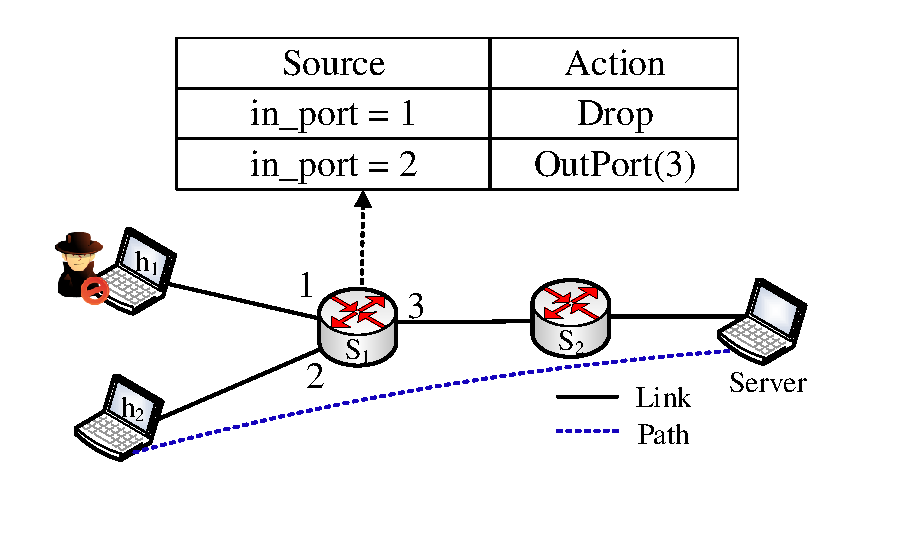
\includegraphics[width=3.4in]{Design/defense.pdf}
\vspace{-0.1in}
\caption{\small{An example of our defense. The low-rate TCP attack from $h_1$ overload the bandwidth of the link between $S_2$ and $S_3$. The attack from $h_1$ is mitigated at $S_1$.}}
\label{fig:mitigate}
\vspace{-0.2in}
\end{figure}


